\documentclass{article}

\usepackage{fancyhdr}
\usepackage{extramarks}
\usepackage{amsmath}
\usepackage{amsthm}
\usepackage{amsfonts}
\usepackage{tikz}
\usepackage[plain]{algorithm}
\usepackage{algpseudocode}
\usepackage{dsfont}
\usepackage{subcaption}
\usepackage{lipsum}
\usepackage{ragged2e}
\usepackage{afterpage}

\usetikzlibrary{automata,positioning}

%
% Basic Document Settings
%

\usepackage{graphicx, url}
\graphicspath{figures/}

\topmargin=-0.45in
\evensidemargin=0in
\oddsidemargin=0in
\textwidth=6.5in
\textheight=9.0in
\headsep=0.25in

\linespread{1.1}

\pagestyle{fancy}

% The page Header
\lhead{\hmwkAuthorName}
\chead{\hmwkClassShort}
\rhead{\hmwkTitle}
\lfoot{\lastxmark}
\cfoot{\thepage}

\renewcommand\headrulewidth{0.4pt}
\renewcommand\footrulewidth{0.4pt}

\setlength\parindent{0pt}

%
% Create Problem Sections
%

\newcommand{\enterProblemHeader}[1]{
    \nobreak\extramarks{}{Problem \arabic{#1} continued on next page\ldots}\nobreak{}
    \nobreak\extramarks{Problem \arabic{#1} (continued)}{Problem \arabic{#1} continued on next page\ldots}\nobreak{}
}

\newcommand{\exitProblemHeader}[1]{
    \nobreak\extramarks{Problem \arabic{#1} (continued)}{Problem \arabic{#1} continued on next page\ldots}\nobreak{}
    \stepcounter{#1}
    \nobreak\extramarks{Problem \arabic{#1}}{}\nobreak{}
}

\setcounter{secnumdepth}{0}
\newcounter{partCounter}
\newcounter{homeworkProblemCounter}
\setcounter{homeworkProblemCounter}{1}
\nobreak\extramarks{Problem \arabic{homeworkProblemCounter}}{}\nobreak{}

%
% Homework Problem Environment
%
% This environment takes an optional argument. When given, it will adjust the
% problem counter. This is useful for when the problems given for your
% assignment aren't sequential. See the last 3 problems of this template for an
% example.
%
\newenvironment{homeworkProblem}[1][-1]{
    \ifnum#1>0
        \setcounter{homeworkProblemCounter}{#1}
    \fi
    \section{Problem \arabic{homeworkProblemCounter}}
    \setcounter{partCounter}{1}
    \enterProblemHeader{homeworkProblemCounter}
}{
    \qed
    \exitProblemHeader{homeworkProblemCounter}
}

%
% Homework Details
%   - Title
%   - Due date
%   - Class
%   - Section/Time
%   - Instructor
%   - Author
%

\newcommand{\hmwkTitle}{Homework 3}
\newcommand{\hmwkDueDate}{May, 21}
\newcommand{\hmwkClassShort}{AMATH 563 }
\newcommand{\hmwkClass}{\hmwkClassShort \\ Inferring Structure of Complex Systems}
\newcommand{\hmwkClassTime}{Section A}
\newcommand{\hmwkClassInstructor}{Prof. J. Nathan Kutz}
\newcommand{\hmwkAuthorName}{\textbf{Alexey Sholokhov}}
\newcommand{\hmwkAuthorEmail}{\textit{aksh@uw.edu}}
\newcommand{\hmwkAbstract}{In this assignment we utilize deep neural networks for predicting the behavior of three different dynamic systems: Lorenz equation, Kuramoto-Sivashinsky Equation and a reaction-diffusion equation. We show that, being properly tuned, this model family demonstrates good prediction quality, although it does not allow us to reconstruct the original governing equation.}

%
% Title Page
%

\title{
%    \vspace{2in}
    \textmd{\textbf{\hmwkClass\\\ \hmwkTitle}}\\
    \normalsize\vspace{0.1in}\small{Due\ on\ \hmwkDueDate\ at 23:59}\\
    \vspace{0.1in}\large{\textit{\hmwkClassInstructor}}
%    \vspace{1in}\\
    \justify{\textbf{Abstract: }\hmwkAbstract}
%    \vspace{1in}
}


\author{\hmwkAuthorName\\ \hmwkAuthorEmail}
\date{\today}

\renewcommand{\part}[1]{\textbf{\large Part \Alph{partCounter}}\stepcounter{partCounter}\\}

%
% Various Helper Commands
%

% Useful for algorithms
\newcommand{\alg}[1]{\textsc{\bfseries \footnotesize #1}}

% For derivatives
\newcommand{\deriv}[1]{\frac{\mathrm{d}}{\mathrm{d}x} (#1)}

% For partial derivatives
\newcommand{\pderiv}[2]{\frac{\partial}{\partial #1} (#2)}

% Integral dx
\newcommand{\dx}{\mathrm{d}x}

% Alias for the Solution section header
\newcommand{\solution}{\paragraph{Solution} }

% Probability commands: Expectation, Variance, Covariance, Bias
\newcommand{\Var}{\mathrm{Var}}
\newcommand{\Cov}{\mathrm{Cov}}
\newcommand{\Bias}{\mathrm{Bias}}
\newcommand*{\pd}[3][]{\ensuremath{\frac{\partial^{#1} #2}{\partial #3}}}
\newcommand*{\prob}[1]{\ensuremath{\mathbb{P}\left[#1\right]}}
\newcommand*{\ind}[1]{\ensuremath{\mathds{1}_{\left[#1\right]}}}
\newcommand*{\at}[2]{\Big|_{#1}^{#2}}

%
% Different math operators
\DeclareMathOperator{\dom}{Dom}
\DeclareMathOperator{\diag}{Diag}
\DeclareMathOperator{\prox}{prox}
\DeclareMathOperator*{\proj}{proj}
\DeclareMathOperator*{\sign}{sign}
\DeclareMathOperator*{\argmax}{argmax}
\DeclareMathOperator*{\argmin}{argmin}

%% \mathbb symbols
\DeclareMathOperator{\E}{\mathbb{E}}
\DeclareMathOperator{\A}{\mathbb{A}}
\DeclareMathOperator{\R}{\mathbb{R}}
\DeclareMathOperator{\X}{\mathbb{X}}
\DeclareMathOperator{\N}{\mathbb{N}}
\DeclareMathOperator{\Q}{\mathbb{Q}}

%% \mathcal symbols
\DeclareMathOperator{\RR}{\mathcal{R}}
\DeclareMathOperator{\PP}{\mathcal{P}}
\DeclareMathOperator{\NN}{\mathcal{N}}
\DeclareMathOperator{\CC}{\mathcal{C}}
\DeclareMathOperator{\FF}{\mathcal{F}}
\DeclareMathOperator{\YY}{\mathcal{Y}}



\begin{document}

\maketitle
\section{Introduction}
Neural network models is a broad family of nonlinear models which have found applications in various domains, from biology to image analysis, stock price prediction, robotics and many others. Several extensions of this model family have been invented over the last 20 years, such as Convolutional, Recursive, and Adversarial networks. However, the flexibility of these models comes with the price of excessive amount of hyper parameters to choose, such as the number of layers, their type, their activation functions, and the number of perceptrons and channels for each layer. Nevertheless, these models, being properly tuned, are well known for providing outstanding results in classification, regression, time series prediction, and dynamical system simulation problems. In this work we focus on the later domain of application, utilizing deep neural networks for predicting the behavior of three dynamical models: Lorenz system, Kuramoto-Sivashinsky equation, and a reaction-diffusion equation. 

\section{Theoretical Background}
\paragraph{Model Discovery with Neural Networks}
Consider a dynamic model 
    \begin{equation}
    \label{eq:general_dynamic_model}
        u_t = f(u(x,t)), \quad x \in \R^d, \, t \in \R_+
    \end{equation}
    where the governing equation $f(u, t)$ is unknown. Our goal is to model the behavior of the system using a set of data measurements 
    \[
        U = \{(x_i, t_i, u(x_i, t_i)\}_{i=1}^{m}
    \]
    
    We do not make any assumptions on the structure of $f$, as we did in the previous homework while using the CINDy framework. The same time, we have no goal to reconstruct the right hand-side of the equation \ref{eq:general_dynamic_model}: the goal is to build a model which predicts the next step in the best way possible. 
        
    \paragraph{Neural Networks}
    The family of models we consider in this work are Neural Networks (NNs). The elemental building block of Neural Networks is a perceptron, which is defined as:
    \begin{equation}
        \label{eqn:lorentz}
        y = f\left(\sum_{i = 1}^nx_iw_i + w_0\right)    
    \end{equation}
    where $x_i$ are the coordinates of an input vector, $y$ is the perceptron's output, and $f(x)$ is called the activation function. A simplest Neural Network consists of two fully connected layers of perceptrons (input and output). If the NN has more than two layers it's called Deep Neural Network. One may check \cite{deeplearningbook} for further details.
    \paragraph{Lorenz system} A Lorentz dynamic system is defined as a system of ODEs
    \begin{equation}
        \frac{dx}{dt} = \sigma(y-x), \quad \frac{dy}{dt} = x(\rho - z) - y, \quad \frac{dz}{dt} = xy-\beta z
    \end{equation}
    
    \paragraph{Kuramoto-Sivashinsky equation} The Kuramoto-Sivashinsky equation is a PDE of the following form
    \begin{equation}
        u_t + \nabla^4u + \nabla^2u + \frac{1}{2}|\nabla u|^2 = 0
    \end{equation}
    It models the diffusive instabilities in a laminar flame front, see \cite{KS} for details. 

    \paragraph{Reaction-Diffusion equation} A reaction-diffusion equation is a model which commonly describes the change in concentration of one or more chemical substances over time and space
    \begin{equation}
        u_t = \diag{(\nabla^2u)} + R(u)
    \end{equation}

\begin{figure}
    \centering
    \begin{subfigure}[b]{0.4\textwidth}
        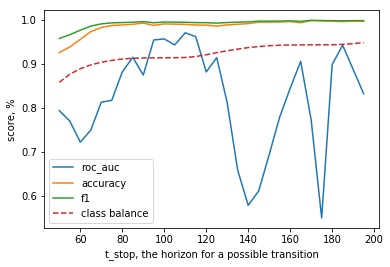
\includegraphics[width=\textwidth]{images/lorentz_lobes_transition}
        \caption{Lorenz lobe transition prediction \label{fig:lorenz_lobes}. We see that the prediction quality (ROC AUC) increases when class imbalance is less than 0.9, then the prediction quality becomes unstable. }
    \end{subfigure}\hspace{5mm}%
    \begin{subfigure}[b]{0.4\textwidth}
        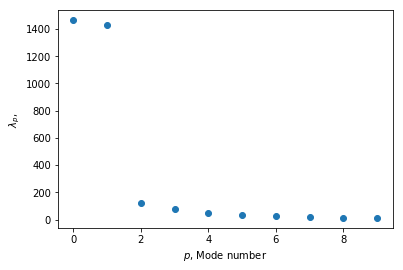
\includegraphics[width=\textwidth]{images/rd_spectre}
        \caption{The spectre of reaction diffusion data. First four modes carry the vast majority of the variance in data, so defining the truncation rank $r = 4$ seems reasonable.\label{fig:rd_spectre}}
    \end{subfigure}
\end{figure}


\section{Algorithm Implementation and Development}

\begin{figure}
    \centering
    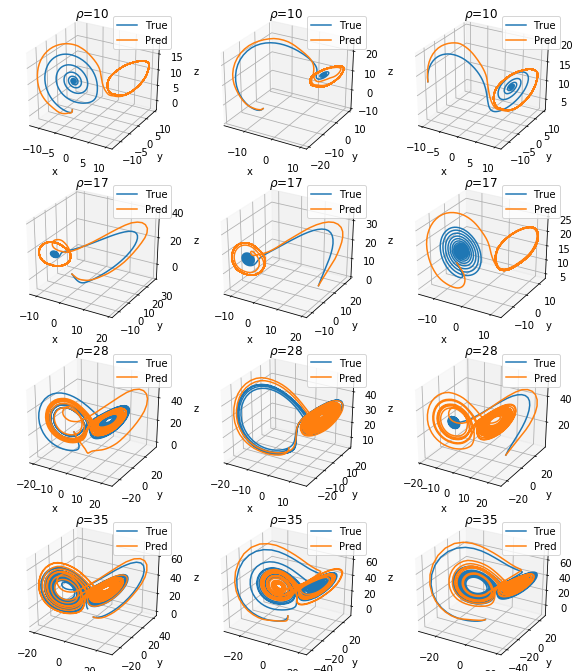
\includegraphics[width=\textwidth]{images/lorentz_trajectories}
    \caption{\label{fig:lorentz_trajectories} Predictions of Lorentz oscillation sample trajectories for different $\rho$. We see that the prediction quality for trajectories with $\rho = 17,\, 35$ which were not a part of the dataset is almost the same as for $\rho = 10, 28$, which samples were in the training data. It evidences the fact that the model managed to derive the general the pattern of a dynamic systems' behaviour and is not overfitted. }
\end{figure}

\afterpage{%
\begin{figure}
\centering
    \begin{subfigure}[b]{0.9\textwidth}
        \centering
        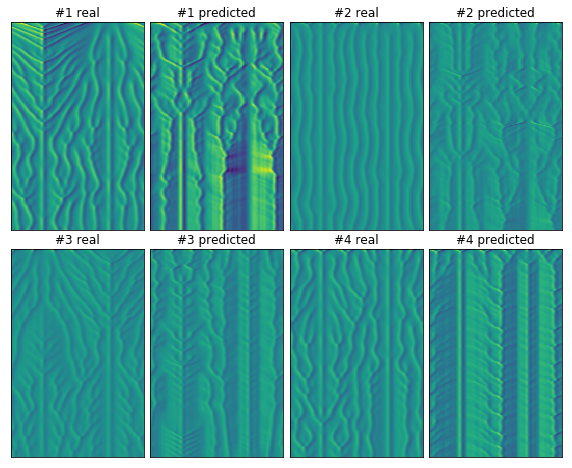
\includegraphics[width=0.7\textwidth, height=0.4\textheight]{images/ks_results}
        \caption{The KS equation modeling results. Wee see that, although the predictions do not math pixel-wise with the originals, the model captures the textural pattern and produces continuous lines. Hence, one could admit that a multi-input CNN was an appropriate architecture for this problem.\label{fig:ks}} 
    \end{subfigure}
    \begin{subfigure}[b]{\textwidth}
        \centering
        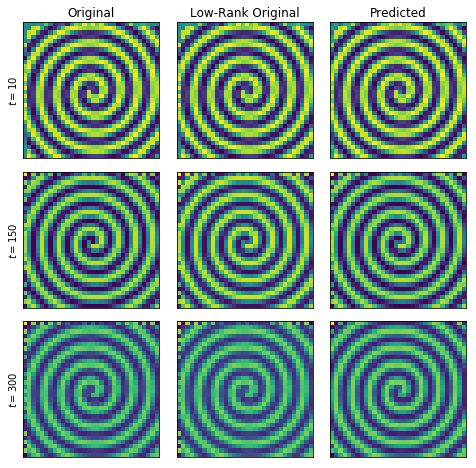
\includegraphics[width=0.7\textwidth]{images/rd_results}
        \caption{The results for the reaction-diffusion modeling. We see that both low rank approximation and the prediction pictures are very similar to the original one, which means that the chosen truncation rank was appropriate.\label{fig:rd}}
    \end{subfigure} 
\end{figure}
}

This section supplements and clarifies the Jupyter Notebook with the code attached to this homework 

 
\paragraph{Section 1.1} The first section is devoted to the modeling of trajectories of Lorentz system (Eq. \ref{eqn:lorentz}) . 
    \begin{enumerate}
    \item[1)] We generate a dataset by sampling random initial points $x_0 \in U[0,30]^3 \subset \R^3$ and calculating the respective trajectories with \texttt{numpy.integrate.solve\_ivp} routine. For each $\rho \in [10, 28, 40]$ we generate 100 random trajectories and then split this data between variables \texttt{x\_train} and \texttt{y\_train} in the proportion of 80 to 20 respectively. 
    \item[2)] We define \texttt{Lorentz\_1step}: a three-layer DNN for predicting next step along the trajectory basing on a previous one (see table \ref{table:nets}). We train it on \texttt{(x\_train, y\_train)} data and use \texttt{(x\_test, y\_test)} data as a validation dataset. 
    \item[3)] We visualize the test results of the model by plotting three random trajectories (real and predicted) for each $\rho \in [10, 17, 28, 35]$, see figure \ref{fig:lorentz_trajectories}. 
    \end{enumerate}
\paragraph{Section 1.2} In this section we train a model for predicting whether the transition between lobes for a trajectory from a given starting point is imminent. 
    \begin{enumerate}
        \item[1)] We generate a dataset: a set of starting points \texttt{x\_train\_lobes} with times \texttt{t\_train\_lobes} when the respective trajectory crosses the plane between lobes ($x = 0$) for the first time. 
        \item[2)] In order to establish for how far in advance we can predict whether the transition will happen we iterate over $\texttt{t\_stop} \in [50, 250]$ and define \texttt{y\_train\_lobes} as \texttt{[t\_train\_lobes <= t\_stop]}. In other words, if the transition happens after the $\texttt{t\_stop}$ we say that the transition will not happen (\texttt{y\_train\_lobes = 0}) and that it's imminent otherwise (\texttt{y\_train\_lobes = 1})). For each pair (\texttt{x\_train\_lobes}, \texttt{y\_train\_lobes}) we train a DNN \texttt{Lorentz\_lobes}, see the architecture in the Table \ref{table:nets} and measure its accuracy, F1-measure, and ROC-AUC score. These metrics and the balance between classes are presented in the Figure \ref{fig:lorenz_lobes}. 
    \end{enumerate}
\paragraph{Section 2} In this section we model the dynamics of Kuramoto-Sivashinsky(KS) equation.
    \begin{enumerate}
        \item[1)] We generate a dataset of 1000 KS solutions with random initial conditions of the form 
            \[
                u_0(x) = \alpha \cos(2\pi \beta x/16)(1+\sin(2\pi\beta x/16)), \quad \alpha \in \R, \quad \beta, \gamma \in \N_+
            \]
            Arrays \texttt{x\_train\_kse} and \texttt{y\_train\_kse}, defined as in the previous section. In addition, for each row in \texttt{x\_train\_kse} we save the array of initial parameters [$\alpha$, $\beta$, $\gamma$], with which this row was generated. 
        \item[2)] We define \texttt{model\_KSE} -- a 1D convolutional multi-input DNN, see the architecture in the Table \ref{table:nets} .To understand the motivation behind note that both FDE stencils and convolutions w/o activation are linear functions of local neighborhoods, so the first convolutional layer is intended to approximate finite difference schemes, which would provide a good solution with just one layer, if it were possible to find them. However, it is barely possible in practice, so we add couple of extra dense layers for better approximation. Second, our feature space is heterogeneous, and it makes no sense to convolve data with initial parameters, so instead of just attaching parameters to the input vector we attach them separately after the first convolutional layer. 
        \item[3)] The MSE error does not represent the performance of the model in this case, so we visualize six random solutions (fig. \ref{fig:ks}) to assess the model's performance. 
    \end{enumerate}

\paragraph{Section 3} This section is devoted to the modeling of reaction-diffusion equation solution. 
    \begin{enumerate}
        \item[1)] We generate one sample solution with $L=50$, evaluate it on a grid of 8192 points, stretch all pictures to vectors, and store it in \texttt{x\_train\_rd} array. The target set \texttt{y\_train\_rd} is defined as \texttt{x\_train\_rd} shifted one step further in time. 
        \item[2)] In order to reduce the dimensionally of data, we analyze its dominant modes, see the picture \ref{fig:rd_spectre}. We then project the data in low-dimensional space using SVD decomposition.
        \item[3)] Due to low dimensionality of data we use \texttt{model\_RD} a simple two-layer feed-forward DNN with two hidden layers, see the architecture in \ref{}.
        \item[4)] To assess the model's quality we reconstruct the test part of data using our model and then compare three snapshots with the real solution for $t \in [10, 150, 300]$ (Fig. \ref{fig:rd}).  
    \end{enumerate}

\section{Computational Results}
    In this section we discuss numerical results specifically addressing parts of the assignment.
    \subsection{Lorentz Equation} Sample trajectories which were reconstructed with our model are depicted in the figure \ref{fig:lorentz_trajectories} . It's clear that the model does not always work perfectly, but it captures the main "butterfly" pattern of trajectories and reconstruct trajectories with $\rho = 17$ and $\rho = 35$ adequately, although they have not been in the training dataset. 
    \subsection{Kuramoto-Sivashinsky Equation} The six random KS equation trajectories reconstructed by the model are in the figure \ref{fig:ks}. It's clear that the NN has captured  textural patterns of the solution (pictures 2 and 3). The same time, original and predicted samples are apparently not point-wise similar, however, it strongly depends on  random parameters both in initial conditions and the model's weight initialization (see the fig. \ref{fig:ks_extra} in Appendix A for prettier samples). Also, we see that the predicted solution tends to stuck in a cyclic pattern unrelated to the original picture, like in examples 1, 4). One explanation of why it happens could happen is that the model accumulates errors from the previous steps affecting future predictions, and, comparing to FDMs, we have no bounds for this error. 
    \subsection{Reaction-Diffusion Equation} 
    On the figure \ref{fig:rd_spectre} one may see the absolute singular values of the data. Almost the variance of the data is concentrated in the first two singular values, so the truncation rank $r  = 4$ seems reasonable. Three random time snapshots of the original, truncated and predicted reaction in U are presented in the Figure \ref{fig:rd}. We see that the model predicts the reaction's behavior adequately, which means that the rank truncation was too strong. We see that forecasting in the low-rank space works better: comparing to the KS equation, the reaction-diffusion part required much simpler network model took significantly lesser time to train.     

\section{Summary and Conclusion}
    In this work we applied Deep Neural Networks for modeling of three different types of equations. We showed that these models, being properly tuned, provide sufficient accuracy of the solution and capture general patterns of undergoing reactions. The main drawback here is that the resulting models are not interpretable, hence we can not reconstruct the original RHS of the dynamical system, as it was possible with CINDy. 


\begin{thebibliography}{99}

\bibitem{KS} Sivashinsky, G. S. (1977). Nonlinear analysis of hydrodynamic instability in laminar flames—I. Derivation of basic equations. In Dynamics of Curved Fronts (pp. 459-488).
\bibitem{deeplearningbook}Ian Goodfellow and Yoshua Bengio and Aaron Courville "Deep Learning", MIT Press, 2016, \url{http://www.deeplearningbook.org}
\end{thebibliography}

\newpage
\section{Appendix A: code references and extra materials}
\begin{enumerate}
    \item \texttt{tensorflow} -- a library for numerical computations on directed acyclic computational graphs and machine learning see \url{https://www.tensorflow.org}
    \item \texttt{keras} -- a high-level neural network API, see \url{https://keras.io}
\end{enumerate}

\begin{table}[h!]
    \centering
    \begin{tabular}{c|c|c|c}
        \texttt{Lorentz\_1step} & \texttt{Lorentz\_lobes} & \texttt{model\_RD} & \texttt{model\_KSE} \\ 
        \hline
        Input(4) & Input(3) & Input(4)& Input1(128) \\
        Dense(50) & Dense(30) & Dense(20)& Conv1D(4, 3)[Input1] \\
        Activation(ReLu) & Activation(Sigmoid)& Activation(Tanh)& Input2(3) \\
        Dense(30) & Dense(30)& Dense(20)& Dense(3)[Input2]\\
        Activation(ReLu) & Activation(Sigmoid) & Activation(Tanh)& Flatten()[Conv1D] \\
        Dense(30) & Dense(30) & Dense(20)& Concatenate()[Dense, Flatten] \\
        Activation(ReLu) & Activation(Sigmoid) & Activation(Tanh)& Dense(256) \\
        Dense(3) & Dense(1) & Dense(4)& Activation(Tanh)\\    
        Activation(Linear) & Activation(Sigmoid) & Activation(Linear)& Dense(128)\\
    \end{tabular}
\caption{Architectures of Neural Networks used in this assignment\label{table:nets}}
\end{table}

\begin{figure}[h!]
    \centering
    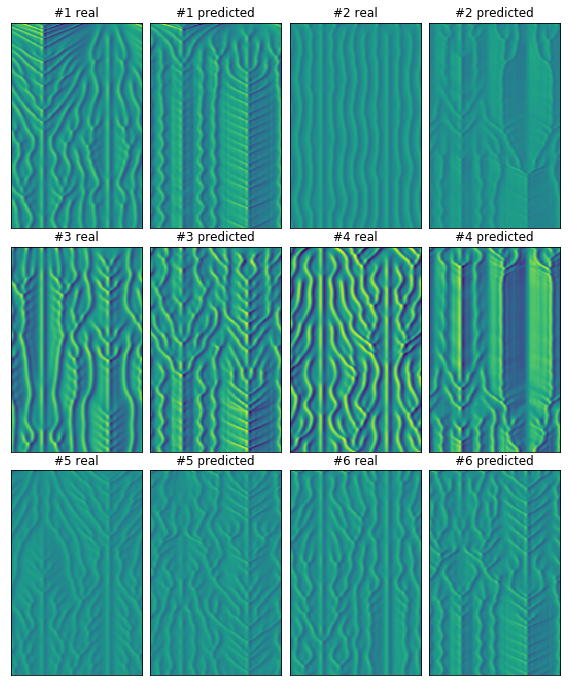
\includegraphics[width=0.6\textwidth]{images/ks_extras}
    \caption{More samples for the Kuramoto-Sivashinsky system \label{fig:ks_extra}}
\end{figure}

\end{document}
